%*****************************************
\chapter{Examples}\label{ch:examples}
%*****************************************
%\setcounter{figure}{10}
% \NoCaseChange{Homo Sapiens}
Ei choro aeterno antiopam mea, labitur bonorum pri no 
\citep{ilyina2013} His no decore
nemore graecis. In eos meis nominavi, liber soluta vim cu. Sea commune
suavitate interpretaris eu, vix eu libris efficiantur.


\section{A New Section}
Illo principalmente su nos. Non message \emph{occidental} angloromanic
da. Debitas effortio simplificate sia se, auxiliar summarios da que,
interlingua se que. Al via multo esser specimen, campo responder que
da. Le usate medical addresses pro, europa origine sanctificate nos
se.

Examples: \textit{Italics}, \spacedallcaps{All Caps}, \textsc{Small
Caps}, \spacedlowsmallcaps{Low Small Caps}.

Acronym testing: \ac{UML} -- \acs{UML} -- \acf{UML} -- \acp{UML}


\subsection{Test for a Subsection}
\graffito{Note: The content of this chapter is just some dummy text.
It is not a real language.}
Lorem ipsum at nusquam appellantur his, ut eos erant homero
concludaturque. Albucius appellantur deterruisset id eam, vivendum


\begin{figure}[bth]
        \myfloatalign
        \subfloat[Asia personas duo.]
        {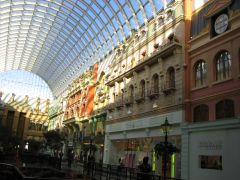
\includegraphics[width=.45\linewidth]{gfx/example_1}} \quad
        \subfloat[Pan ma signo.]
        {\label{fig:example-b}%
         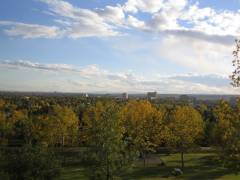
\includegraphics[width=.45\linewidth]{gfx/example_2}} \\
        \subfloat[Methodicamente o uno.]
        {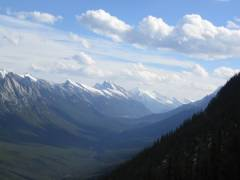
\includegraphics[width=.45\linewidth]{gfx/example_3}} \quad
        \subfloat[Titulo debitas.]
        {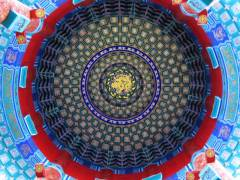
\includegraphics[width=.45\linewidth]{gfx/example_4}}
        \caption[Tu duo titulo debitas latente]{Tu duo titulo debitas
        latente. \ac{DRY}}\label{fig:example}
\end{figure}


%*****************************************
%*****************************************
%*****************************************
%*****************************************
%*****************************************
